Next, we discuss the method for obtaining the $\bar{K}N$ pole parameters through fitting under the assumption of a 2-step reaction.
This approach is similar to that used by Noumi et el., as introduced in Chapter 1.
Since this analysis method focuses only on $I=0$, the obtained spectra are separated into components of $I=0$.
In this procedure, the spectra are further separated into components of $I=1$ and, in addition, the interference term between $I=0$ and $I=1$.
The obtained spectrum can be expressed as follows from the isospin relation.

\newcommand{\Tmat}{T_{\bar{K}N \rightarrow \pi \Sigma}}
\newcommand{\Cfirst}{C_{K^- N \rightarrow \bar{K}N}}
\newcommand{\CS}{\frac{d\sigma}{d\Omega dM}}
\begin{align}
  \CS(\pi^\mp \Sigma^\pm) \propto & \left| \Cfirst^0 \Tmat^{I=0} \mp \Cfirst^1 \Tmat^{I=1} \right|^2 \nonumber \\
  = & \left| \Cfirst^0 \Tmat^{I=0} \right|^2 + \left| \Cfirst^1 \Tmat^{I=1} \right|^2 \nonumber \\
    & \mp 2\mbox{Re}( \Cfirst^0 \Cfirst^1 \Tmat^{I=0} \Tmat^{I=1} ) & \label{eq:Charge_piS} \\
  \CS(\pi^- \Sigma^0) \propto & \left| \Cfirst^1 \Tmat^{I=1} \right|^2 \label{eq:pimS0}
\end{align}

Here, $\Tmat^{I=0,1}$ represents the $T$ matrix of the second $\bar{K}N \rightarrow \pi \Sigma$ scattering for isospin $I=0$ and $I=1$.
Additionally, $\Cfirst^{0,1}$ denotes the factor for the first $K^- p \rightarrow \bar{K}N$ scattering,
corresponding to the isospin $I=0$ and $I=1$ components of the second scattering.

Since it can be expressed as shown in Equation (\ref{eq:Charge_piS}), (\ref{eq:pimS0}),
the spectra corresponding to $I=0$, $I=1$, and their interference terms can be written as follows.
\begin{align}
  & \CS(I=0) \propto \frac{1}{2}\left( \CS(\pi^- \Sigma^+)+\CS(\pi^+ \Sigma^-)-\CS(\pi^-\Sigma^0) \right) \label{eq:I0}\\
  & \CS(I=1) \propto \CS(\pi^- \Sigma^0) \label{eq:I1}\\ 
  & \CS(int) \propto \left( \CS(\pi^- \Sigma^+)-\CS(\pi^+\Sigma^+) \right) \label{eq:interfer}
\end{align}

\begin{figure}[htbp]
  \centering
  \begin{tabular}{ccc}
    \begin{minipage}{0.33\hsize}
      \includegraphics[width=4cm]{../pic/Dron/fit_I0_KzeroN.eps}
    \end{minipage}
    \begin{minipage}{0.33\hsize}
      \includegraphics[width=4cm]{../pic/Dron/fit_I0_KN.eps}
    \end{minipage}
    \begin{minipage}{0.33\hsize}
      \includegraphics[width=4cm]{../pic/Dron/fit_I0_Kmp.eps}
    \end{minipage}
  \end{tabular}
  \begin{tabular}{ccc}
    \begin{minipage}{0.33\hsize}
      \includegraphics[width=4cm]{../pic/Dron/fit_scat_amp_I0_KzeroN.eps}
    \end{minipage}
    \begin{minipage}{0.33\hsize}
      \includegraphics[width=4cm]{../pic/Dron/fit_scat_amp_I0_KN.eps}
    \end{minipage}
    \begin{minipage}{0.33\hsize}
      \includegraphics[width=4cm]{../pic/Dron/fit_scat_amp_I0_Kmp.eps}
    \end{minipage}
  \end{tabular}
  \caption{
    This figure shows the $I=0$ spectrum obtained from Eq. (\ref{eq:I0}) and the fit results assuming a 2-step reaction.
    In the upper panel, the error bars represent the experimental data, the red line indicates the spectrum resulting from the fit,
    the solid line corresponds to the spectrum convolved with detector resolution, and the dashed line represents the spectrum without resolution.
    The lower panel displays the scattering amplitude for the two-step $\bar{K}N \rightarrow \bar{K}N$ scattering,
    where the red line indicates the real part and the blue line shows the imaginary part.
    The lines are the best-fit values and the bands hatched in color represent the width of the error due to fitting.
  }
  \label{fig:fit_2step_I0}
\end{figure}


The 2-step response can be expressed as follows,
\begin{equation*}
   \frac{d\sigma}{dM_{\pi\Sigma}d\Omega_{n}}
   =\left| \bra{n_{\theta=0}\pi\Sigma} T^2_{\bar{K}N_2 \rightarrow \pi \Sigma}
   G_0(\bar{K}, N_2) T^1_{K^-N_1 \rightarrow \bar{K} N} \ket{K^-\Phi_{d}} \right|^2 
\end{equation*}
where $G_0(\bar{K}, N_2)$, represents the Green's function describing the propagation of virtual $\bar{K}$ mesons
between the first and second scattering steps.
This equation can be factorized using the deuterium wavefunction $\psi_d(p)$ and decomposed into
a 1-step response $f_{res}(M_{\pi \Sigma})$function and a 2-step scattering amplitude as shown below.
\begin{align*}
   & \frac{d\sigma}{dM_{\pi\Sigma}d\Omega_{n}}
     \sim \left| T^2_{\bar{K}N_2 \rightarrow \pi \Sigma} \right|^2 F_{res}(M_{\pi \Sigma}) \\
   & F_{res}(M_{\pi \Sigma}) = \left| \int G_0(\bar{K}, N_2) T^1_{K^-N\rightarrow \bar{K}N} \psi_d(p) d^3p_{N} \right|^2
\end{align*}
The $T$-matrix of the second scattering is expressed as follows, utilizing the low-energy expansion up to the second order for the two channels
\cite{Lensniak}.
\begin{align*}
   & T^2_{\bar{K} N \rightarrow \bar{K}N} = \frac{A}{1-iA k_2+\frac{1}{2}A Rk_2^2}\\
   & T^2_{\bar{K} N \rightarrow \pi \Sigma} =
   \frac{e^{i\delta}}{\sqrt{k_1}}\frac{\sqrt{{\bf Im}A-\frac{1}{2}|A|^2{\bf Im}Rk_2^2}}{1-iAk_2+\frac{1}{2}ARk_2^2}
\end{align*}

This fit includes the scattering length $A$ and the effective range $R$ of the second-step scattering,
along with a parameter determining the overall scale.
In other words, the shape of the first-step scattering (reaction function) is fixed,
and the spectrum shape is determined solely by the second-step scattering.
The scattering length and effective range are complex numbers, so there are five free parameters in total.
This fitting is performed using three $\bar{K}N$ threshold values: $K^- p$, $\bar{K}N$ (the average of $K^- p$ and $K^0 n$), and $K^0 n$.
The discrepancies in the results arising from the differences in threshold values are evaluated as a source of systematic error.
These differences in threshold values are reflected not only in the mass of the $\bar{K}N$ channel in the $T$-matrix of the seccond-scattering
but also in the mass of the nucleon used to calculate the response function in the first-step scattering.
The figure above shows the results of the fit: black error bars represent the data,
and the red solid line shows the fit results convolved with detector resolution, which are used to calculate the chi-square.
The red dashed line shows the fit spectrum without detector resolution,
and the blue dashed line indicates the response function, scaled arbitrarily.
The figure below shows the scattering amplitude obtained from the fit, with red and blue representing the real and imaginary parts, respectively.
The lines indicate the best-fit result, and the bands show the error range,
determined by the maximum and minimum values when adjusting the real and imaginary parts of $A$ and $R$ within their error margins.
The central values of the parameters and the fitting errors were evaluated in terms of the average $\bar{K}N$ threshold,
with $A = \fitScatLength$ and $R = \fitEffRange$.
These values need to be converted to the pole’s position [MeV] and width [MeV],
where the pole is defined by setting the denominator of the $T$-matrix to zero, i.e., by solving the following equation.
\begin{equation}
\frac{1}{2}ARk^2+Ak^2+1=0 \label{eq:pole}
\end{equation}
Where $k$ is the momentum of the $\bar{K}N$ center-of-mass system, converted to mass by $m=\sqrt{m_{\bar{K}N}^2+k^2}$.

\begin{figure}
  \begin{tabular}{ccc}
    \begin{minipage}{0.33\hsize}
      \includegraphics[width=4cm]{../pic/Dron/fit_L1405_pole_Kmp_5.eps}
    \end{minipage}
    \begin{minipage}{0.33\hsize}
      \includegraphics[width=4cm]{../pic/Dron/fit_L1405_pole_KN_5.eps}
    \end{minipage}
    \begin{minipage}{0.33\hsize}
      \includegraphics[width=4cm]{../pic/Dron/fit_L1405_pole_KzeroN_5.eps}
    \end{minipage}
  \end{tabular}

  \begin{tabular}{ccc}
    \begin{minipage}{0.33\hsize}
      \includegraphics[width=4cm]{../pic/Dron/fit_L1405_pole_Kmp_4.eps}
    \end{minipage}
    \begin{minipage}{0.33\hsize}
      \includegraphics[width=4cm]{../pic/Dron/fit_L1405_pole_KN_4.eps}
    \end{minipage}
    \begin{minipage}{0.33\hsize}
      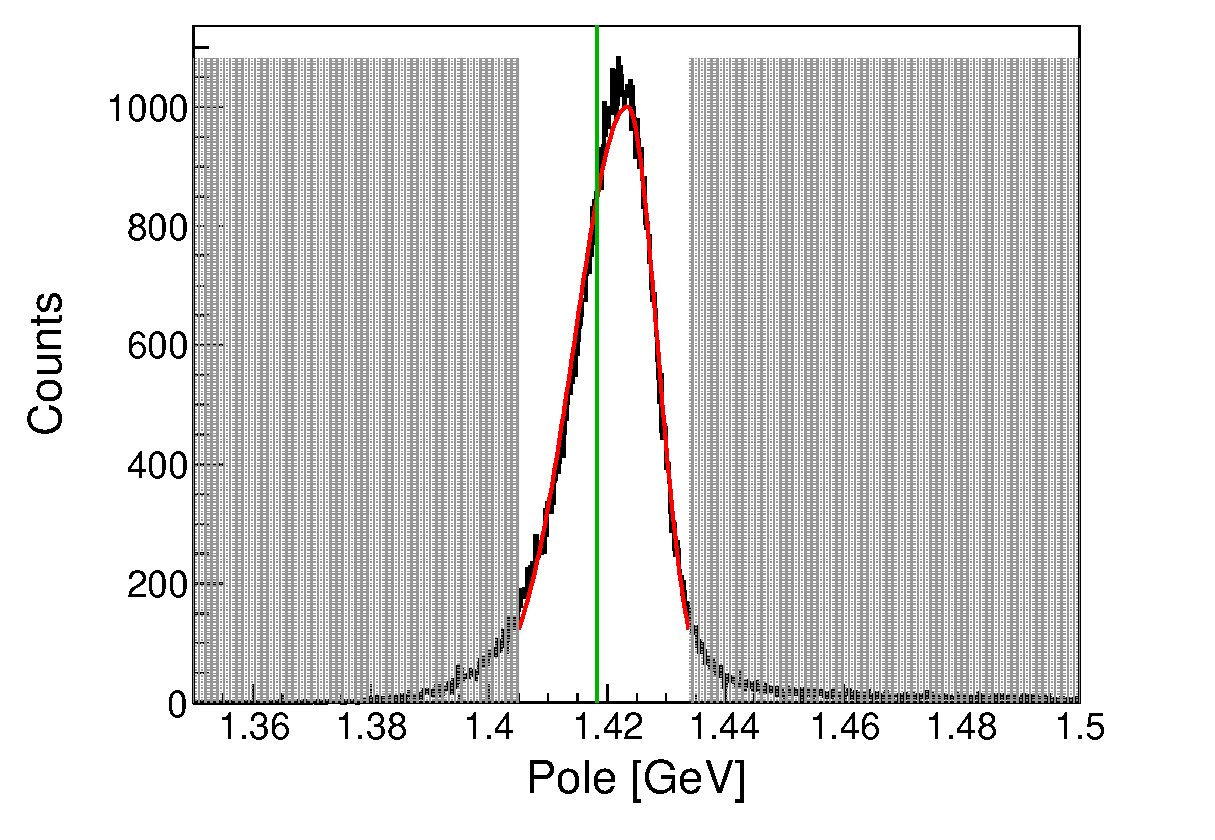
\includegraphics[width=4cm]{../pic/Dron/fit_L1405_pole_KzeroN_4.eps}
    \end{minipage}
  \end{tabular}

  \begin{tabular}{ccc}
    \begin{minipage}{0.33\hsize}
      \includegraphics[width=4cm]{../pic/Dron/fit_L1405_pole_Kmp_3.eps}
    \end{minipage}
    \begin{minipage}{0.33\hsize}
      \includegraphics[width=4cm]{../pic/Dron/fit_L1405_pole_KN_3.eps}
    \end{minipage}
    \begin{minipage}{0.33\hsize}
      \includegraphics[width=4cm]{../pic/Dron/fit_L1405_pole_KzeroN_3.eps}
    \end{minipage}
  \end{tabular}

  \begin{tabular}{ccc}
    \begin{minipage}{0.33\hsize}
      \includegraphics[width=4cm]{../pic/Dron/fit_L1405_pole_Kmp_2.eps}
    \end{minipage}
    \begin{minipage}{0.33\hsize}
      \includegraphics[width=4cm]{../pic/Dron/fit_L1405_pole_KN_2.eps}
    \end{minipage}
    \begin{minipage}{0.33\hsize}
      \includegraphics[width=4cm]{../pic/Dron/fit_L1405_pole_KzeroN_2.eps}
    \end{minipage}
  \end{tabular}

  \begin{tabular}{ccc}
    \begin{minipage}{0.33\hsize}
      \includegraphics[width=4cm]{../pic/Dron/fit_L1405_pole_Kmp_1.eps}
    \end{minipage}
    \begin{minipage}{0.33\hsize}
      \includegraphics[width=4cm]{../pic/Dron/fit_L1405_pole_KN_1.eps}
    \end{minipage}
    \begin{minipage}{0.33\hsize}
      \includegraphics[width=4cm]{../pic/Dron/fit_L1405_pole_KzeroN_1.eps}
    \end{minipage}
  \end{tabular}
  
  \begin{tabular}{ccc}
    \begin{minipage}{0.33\hsize}
      \includegraphics[width=4cm]{../pic/Dron/fit_L1405_pole_Kmp_0.eps}
    \end{minipage}
    \begin{minipage}{0.33\hsize}
      \includegraphics[width=4cm]{../pic/Dron/fit_L1405_pole_KN_0.eps}
    \end{minipage}
    \begin{minipage}{0.33\hsize}
      \includegraphics[width=4cm]{../pic/Dron/fit_L1405_pole_KzeroN_0.eps}
    \end{minipage}
  \end{tabular}
  
  \caption{
    This figure shows the distribution and fit of the poles of $\Lambda(1405)$, generated using Gaussian random numbers.
    The right, center, and left panels correspond to the results based on the $K^- p$, $\bar{K}N$, and $K^0 n$ thresholds, respectively.
    The top row represents the fit over the entire range,
    followed by rows corresponding to the equivalent ranges of $3\sigma$, $2.5\sigma$, $2\sigma$, $1.5\sigma$, and $1\sigma$.
    The fit results are shown as red lines, with gray hatched areas representing regions excluded from the fit.
    The green lines indicate the pole positions corresponding to the best-fit values shown in Figure \ref{fig:fit_2step_I0}.
  }
  \label{fig:fit_L1405_pole}
\end{figure}

\begin{figure}
  \begin{tabular}{ccc}
    \begin{minipage}{0.33\hsize}
      \includegraphics[width=4cm]{../pic/Dron/fit_L1405_width_Kmp_5.eps}
    \end{minipage}
    \begin{minipage}{0.33\hsize}
      \includegraphics[width=4cm]{../pic/Dron/fit_L1405_width_KN_5.eps}
    \end{minipage}
    \begin{minipage}{0.33\hsize}
      \includegraphics[width=4cm]{../pic/Dron/fit_L1405_width_KzeroN_5.eps}
    \end{minipage}
  \end{tabular}

  \begin{tabular}{ccc}
    \begin{minipage}{0.33\hsize}
      \includegraphics[width=4cm]{../pic/Dron/fit_L1405_width_Kmp_4.eps}
    \end{minipage}
    \begin{minipage}{0.33\hsize}
      \includegraphics[width=4cm]{../pic/Dron/fit_L1405_width_KN_4.eps}
    \end{minipage}
    \begin{minipage}{0.33\hsize}
      \includegraphics[width=4cm]{../pic/Dron/fit_L1405_width_KzeroN_4.eps}
    \end{minipage}
  \end{tabular}

  \begin{tabular}{ccc}
    \begin{minipage}{0.33\hsize}
      \includegraphics[width=4cm]{../pic/Dron/fit_L1405_width_Kmp_3.eps}
    \end{minipage}
    \begin{minipage}{0.33\hsize}
      \includegraphics[width=4cm]{../pic/Dron/fit_L1405_width_KN_3.eps}
    \end{minipage}
    \begin{minipage}{0.33\hsize}
      \includegraphics[width=4cm]{../pic/Dron/fit_L1405_width_KzeroN_3.eps}
    \end{minipage}
  \end{tabular}

  \begin{tabular}{ccc}
    \begin{minipage}{0.33\hsize}
      \includegraphics[width=4cm]{../pic/Dron/fit_L1405_width_Kmp_2.eps}
    \end{minipage}
    \begin{minipage}{0.33\hsize}
      \includegraphics[width=4cm]{../pic/Dron/fit_L1405_width_KN_2.eps}
    \end{minipage}
    \begin{minipage}{0.33\hsize}
      \includegraphics[width=4cm]{../pic/Dron/fit_L1405_width_KzeroN_2.eps}
    \end{minipage}
  \end{tabular}

  \begin{tabular}{ccc}
    \begin{minipage}{0.33\hsize}
      \includegraphics[width=4cm]{../pic/Dron/fit_L1405_width_Kmp_1.eps}
    \end{minipage}
    \begin{minipage}{0.33\hsize}
      \includegraphics[width=4cm]{../pic/Dron/fit_L1405_width_KN_1.eps}
    \end{minipage}
    \begin{minipage}{0.33\hsize}
      \includegraphics[width=4cm]{../pic/Dron/fit_L1405_width_KzeroN_1.eps}
    \end{minipage}
  \end{tabular}
  
  \begin{tabular}{ccc}
    \begin{minipage}{0.33\hsize}
      \includegraphics[width=4cm]{../pic/Dron/fit_L1405_width_Kmp_0.eps}
    \end{minipage}
    \begin{minipage}{0.33\hsize}
      \includegraphics[width=4cm]{../pic/Dron/fit_L1405_width_KN_0.eps}
    \end{minipage}
    \begin{minipage}{0.33\hsize}
      \includegraphics[width=4cm]{../pic/Dron/fit_L1405_width_KzeroN_0.eps}
    \end{minipage}
  \end{tabular}
  
  \caption{
    This figure shows the distribution and fit of the widths of $\Lambda(1405)$, generated using Gaussian random numbers.
    The details of the figure caption are identical to those of Figure \ref{fig:fit_L1405_pole}, which provides further context.
  }
  \label{fig:fit_L1405_width}
\end{figure}

\begin{figure}
  \begin{tabular}{cc}
    \begin{minipage}{0.5\hsize}
      \includegraphics[width=7cm]{../pic/Dron/L1405_pole_chi2NDF.eps}
    \end{minipage}
    \begin{minipage}{0.5\hsize}
      \includegraphics[width=7cm]{../pic/Dron/L1405_width_chi2NDF.eps}
    \end{minipage}
  \end{tabular}
  
  \caption{
    This figure illustrates the $\chi^2/NDF$ relationship for the fittings of the $Lambda(1405)$ pole and width,
    as shown in Figures \ref{fig:fit_L1405_pole} and \ref{fig:fit_L1405_width}.
    The left panel corresponds to the pole fittings, while the right panel represents the width fittings.
    The purple, red, and blue lines indicate the results for the $K^- p$, $\bar{K}N$, and $K^0n$ thresholds, respectively.
  }
  \label{fig:L1405_param_chi2NDF}
\end{figure}


Since $A$ and $R$ are complex numbers, propagating their errors is not straightforward.
Therefore, the position and width errors of the poles are estimated by generating a Gaussian distribution
using the real and imaginary parts of $A$ and $R$ as random variables,
with fitting errors as the standard deviation $\sigma$.
This approach is similar to the conventional error propagation method,
which treats each parameter as an independent Gaussian, with the overall error as a composite of Gaussian distributions.
Figure \ref{fig:fit_L1405_pole}, \ref{fig:fit_L1405_width} shows the resulting distribution of position and width.
These distributions are clearly asymmetric, particularly in terms of width, due to a threshold effect caused by the proximity of the thresholds.

\begin{equation*}
  f_{fit}(x)=
  \left\{
    \begin{array}{ll}
      A\exp \left( -\frac{(x-M)^2}{2\sigma_h^2} \right) & (x>M) \\
      A\exp \left( -\frac{(x-M)^2}{2\sigma_l^2} \right) & (x<M)
    \end{array}
  \right.
\end{equation*}

Here, $M$ represents the central value, with $\sigma_h$ and $\sigma_l$ denoting the errors in the high and low regions, respectively.
This function explicitly distinguishes between errors above and below the central value while ensuring continuity at $M$.
%% Here, $M$ represents the central value, with $\sigma_h$ and $\sigma_l$ denoting the errors in the high and low regions, respectively.
%% This function, therefore,
%% has distinct errors in the high and low regions relative to the central value and remains continuous at that central point.
The distribution includes a tail component that deviates from a Gaussian profile, which must be excluded for accurate error evaluation.
%The distribution also appears to include a so-called tail component, which deviates from a Gaussian profile,
% and this component should be excluded to properly evaluate the errors.
To achieve this, the evaluation range is divided into several regions, each corresponding to a percentage of the peak height,
and the fit is performed in each region.
For instance, $\exp\left(-\frac{1}{2}3^2\right)$ corresponds to the $\pm 3 \sigma$ region.
This fitting process was conducted for all regions, ranging from $3\sigma$ to $1\sigma$, with increments of $0.5\sigma$.
Figure \ref{fig:L1405_param_chi2NDF} shows the relationship between the reduced $\chi^2/NDF$ and the cut range for each fit.
Here, the $\chi^2/NDF$ increases from the entire region to $3\sigma$.
This is thought to be due to the limited improvement in the fit because the tail component was not fully removed,
as well as the decrease in $NDF$ resulting from the narrower range.
The $\chi^2/NDF$ seems to reach saturation at the $1.5\sigma$ range.
Therefore, a range of $1.5\sigma$ is chosen as a reference to determine the position and width of the pole of $\Lambda(1405)$,
which is found to be $\fitPole + [\fitWidth]i$ [MeV].
Here, the central value is determined from the scattering length and the effective range of the best fit.
The fitting errors are evaluated using the average of $K^0n$ and $K^-p$ for the threshold values,
and the systematic errors were assessed by varying the threshold values.


